\documentclass[11pt]{beamer}
\usetheme{Madrid}
\usefonttheme{serif}
\definecolor{customcolor}{RGB}{52,25,100} 
\setbeamercolor{structure}{fg=customcolor}

\usepackage[utf8]{inputenc}
\usepackage[T1]{fontenc}

\usepackage{amsmath}
\usepackage{amsfonts}
\usepackage{amssymb}
\usepackage{graphicx}

\DeclareMathOperator{\sen}{sen}
\DeclareMathOperator{\tg}{tg}

\setbeamertemplate{caption}[numbered]

\author[Atishaya Maharjan]{Atishaya Maharjan}
\title{Possible Research Topics USRA 2025}
\newcommand{\email}{maharjaa@umanitoba.ca}
\setbeamertemplate{navigation symbols}{} 
\institute[]{University of Manitoba\par Geometric, Approximation, and Distributed Algorithms (GADA) lab} 
\date{\today} 

\bibliographystyle{apalike}

\begin{document}

\begin{frame}
	\titlepage
\end{frame}

\begin{frame}{Possible Research Topics}
	\tableofcontents
\end{frame}

\section{Geometric Spanning Trees and Hypergraphs that Minimizes the Wiener Index}

\begin{frame}{Wiener Index in Graphs}
	\begin{itemize}
		\item Let $G = (V, E)$ be a weighted undirected graph and let $\delta_G(u, v)$ denote the \textbf{shortest (minimum-weight) path}  between vertices $u$ and $v$ in $G$.
		      \pause
		\item The Wiener index is defined as:
		      \[
			      W(G) = \sum_{u, v \in V} \delta_G(u, v)
		      \]
		      \pause
	\end{itemize}
	\begin{center}
		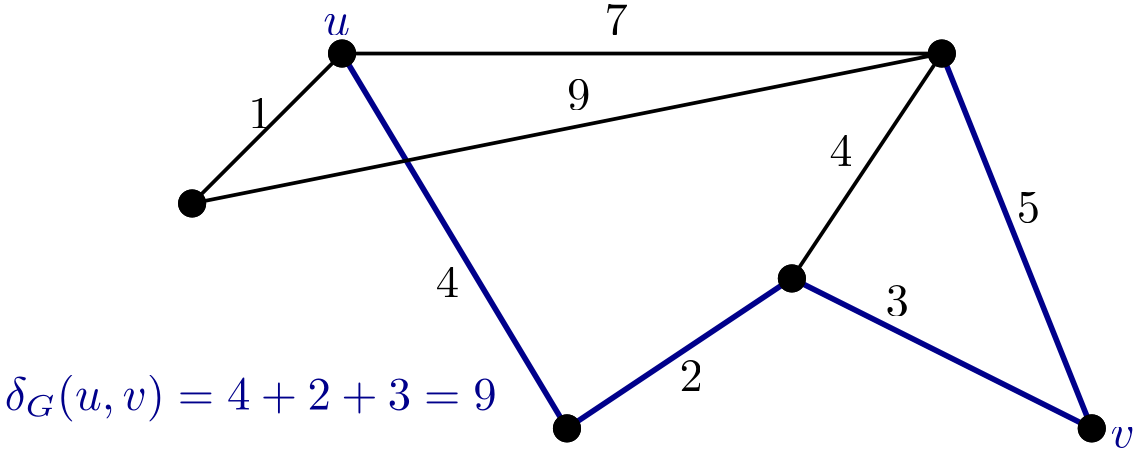
\includegraphics[width=0.75\textwidth]{images/wiener_index.png} % Replace with your own
	\end{center}
\end{frame}

\begin{frame}{Wiener Index in Network Design}
	\begin{itemize}
		\item Given an undirected graph $G = (V, E)$ and a non-negative weight function $w: E \to \mathbb{R}^+$, the goal is to find a spanning tree $T$ of $G$ that minimizes the Wiener index.
		      \pause
		\item The \textbf{routing cost} $c(T)$ of a spanning tree $T$ of $G$ is:
		      \[
			      c(T) = \sum_{u, v \in V} \delta_T(u, v)
		      \]
		      \pause
	\end{itemize}

	\begin{block}{The Minimum Routing Cost Spanning Tree (MRCST) problem}
		\begin{itemize}
			\item Input: A graph $G = (V, E)$ with a non-negative weight function $w: E \to \mathbb{R}^+$.
			\item Output: A spanning tree $T$ of $G$ that minimizes the routing cost $c(T)$.
		\end{itemize}
	\end{block}
	\begin{itemize}
		\pause
		\item The MRCST problem is NP-Complete. There exists a PTAS for MRCST.
	\end{itemize}
\end{frame}

\begin{frame}{Problem Statement: Geometric Spanning Trees}
	\textbf{Reference:} WADS 2023 ~\cite{article:geometric_spanning_trees_minimizing_wiener_index}

	\begin{enumerate}
		\item Input: A set $P$ of $n$ points in the plane.
		      \pause
		\item Goal: Construct a \textbf{spanning tree} on $P$ that minimizes the \textbf{Wiener index}.
		      \pause
		\item The weight function is defined as the Euclidean distance between points.
	\end{enumerate}
\end{frame}

\begin{frame}{Results Summary: Geometric Spanning Trees}
	\begin{itemize}
		\item Spanning tree of $P$ that minimizes the Wiener index is planar.
		      \pause
		\item When $P$ is in convex position, this can be solved in polynomial time.
		      \pause
		\item The hamiltonian path of $P$ that minimizes the Wiener index is not necessarily planar.
		      \pause
		\item Computing such a hamiltonian path is NP-Hard.
	\end{itemize}
\end{frame}

\begin{frame}{Hypergraphs and their Wiener Index}
	\pause
	\begin{block}{Hypergraph}
		A \textbf{hypergraph} $H = (V, E)$ is a pair where $V$ is a set of vertices and $E$ is a set of hyperedges, each of which is a subset of $V$.
	\end{block}

	\pause
	\begin{block}{Distance in Hypergraphs}
		The \textbf{distance} between two vertices $u$ and $v$ in a hypergraph $H$ is defined as the minimum number of hyperedges in a chain connecting $u$ and $v$.
		\begin{itemize}
			\item A \textbf{chain} is a sequence of hyperedges where each consecutive pair shares at least one vertex.
			\item The distance is denoted as $\delta_H(u, v)$.
		\end{itemize}
	\end{block}

	\pause
	\begin{block}{k-uniform hypergraph}
		A hypergraph is \textbf{k-uniform} if every hyperedge has cardinality $k$.
	\end{block}
\end{frame}

\begin{frame}{Wiener Index in Hypergraphs}
	\pause
	\begin{block}{Wiener Index in Hypergraphs}
		The \textbf{Wiener index} of a hypergraph $H$ is defined as:
		\[
			W(H) = \sum_{u, v \in V} \delta_H(u, v)
		\]
	\end{block}
\end{frame}

\begin{frame}{Some facts about HyperGraphs}
	\begin{itemize}
		\pause
		\item Finding a spanning tree of general hypergraphs is NP-Complete, while spanning tree of 3-uniform hypergraphs has a polynomial time algorithm using matroid matching. ~\cite{article:spanning_tree_3_uniform_hypergraph}
		      \pause
		\item Finding a spanning tree of a $k$-uniform 2-regular hypergraph is NP-Complete for any $k \geq 4$. ~\cite{article:spanning_tree_k_uniform_2_regular_hypergraph}
	\end{itemize}
\end{frame}

\begin{frame}{Proposed Open Work: Wiener Index in Hypergraphs}
	\begin{itemize}
		\pause
		\item Focus: Define and study the \textbf{Wiener index} in various classes of hypergraphs.
		      \pause
		\item Distance: Find a suitable weighted/unweighted distance metric for hypergraphs.
		      \pause
		\item Goal: Characterize structures that minimize/maximize the Wiener index.
	\end{itemize}

	\pause
	Side note: We could also explore \textbf{spatially embedded hypergraphs}, drawing inspiration from ~\cite{article:geometric_spanning_trees_minimizing_wiener_index}, and their Wiener index.
\end{frame}

\section{Inside-Out Dissection}

\begin{frame}{Problem Statement: Inside-Out Dissection}
	Reference: Open problem was mentioned in CCCG 2024. \cite{article:inside_out_dissections_polygons_polyhedra} answered the open problem and raised some new questions.

	\pause
	\begin{block}{Inside-out dissection}
		Let $P$ be a polygon (polyhedron). An \textbf{inside-out dissection} of $P$ is a decomposition of $P$ into finitely many polygons (polyhedra) $P_1, \dots, P_k$ such that:
		\begin{itemize}
			\item $P_1, \dots P_k$ can be rearranged by only applying rotations and translations to form a polygon (polyhedron) $P'$ that is congruent to $P$.
			\item The boundary of $P'$ is composed of internal cuts of $P$.
		\end{itemize}
	\end{block}
\end{frame}

%------------------------
\begin{frame}{Visualizing the Problem}
	\pause
	\begin{center}
		Chalk and Talk
	\end{center}
\end{frame}

%------------------------
\begin{frame}{Recent Work Summary}
	\begin{itemize}
		\pause
		\item General n-gon: inside-out dissection possible with at most $2n + 1$ pieces.
		      \pause
		\item Regular polygons (e.g., equilateral triangle, square, regular pentagon): at most 6 pieces suffice.
		      \pause
		\item Extension to 3D:
		      \begin{itemize}
			      \item If a polyhedron can be tiled with regular tetrahedra and octahedra, it can be inside-out dissected.
		      \end{itemize}
		      \pause
		\item Tools used include symmetry arguments and constructive dissections.
	\end{itemize}
\end{frame}

%------------------------
\begin{frame}{Open Work Presented in the Main Reference}
	\begin{itemize}
		\pause
		\item Can a triangle be inside-out dissected with 3 pieces?
		      \pause
		\item Can general $n$-gons be inside-out dissected with lesser than $2n + 1$ pieces? Maybe convex polygons can be done with constant pieces like regular polygons?
		      \pause
		\item They have a method of general polyhedra, but the number of pieces required is quite large. Therefore, an efficient method for inside-out dissections of polyhedra is still open.
	\end{itemize}
\end{frame}

\begin{frame}[allowframebreaks]{References}
	\bibliography{references}
\end{frame}

\begin{frame}

	\begin{center}
		The end.

		\email
	\end{center}

	\begin{figure}[htb]
		\centering
	\end{figure}

\end{frame}

\end{document}
